\documentclass[9pt, xcolor=dvipsnames]{beamer}
\usetheme{Copenhagen}
\setbeamercovered{dynamic}
\usecolortheme[RGB={72,0,4}]{structure} 

%\graphicspath{{immagini/}}
\usepackage{amsmath}
\usepackage[italian]{babel}
\usepackage[utf8x]{inputenc}
\usepackage[T1]{fontenc}
\pgfdeclareimage[height=10mm]{ATLASlogo}{ATLASlogo}
%\logo{\pgfuseimage{logo}}

\usepackage{booktabs}
\usepackage{tabularx}
\usepackage{comment}

\title[Top quark]{Top quark: properties, differences from the other quarks and link to new physics}
%\titlegraphic{\pgfuseimage{ATLASlogo}}
\author[Giuseppe Fasanella]{Candidate: Giuseppe Fasanella}
\institute{Home Institute: ~``Sapienza'' Università di Roma}
\date{ARAP Prize 2013}

\setbeamerfont{section}{family=\rm}
\setbeamertemplate{footline}[frame number]




\begin{document}
\frame{
\titlepage 
}

\begin{frame}
 \frametitle{Overview}
\begin{itemize}
 \item Jet production: considerations
\pause
\bigskip
\item The case of the Top
\pause
\bigskip
\item Coupling to the Higgs bosons
\pause
\bigskip
\item The ttH channel
\end{itemize}
\end{frame}

\begin{frame}
\frametitle{First consideration about jets}
\begin{itemize}
 \item Hadrons are colorless
\item The elementary interaction involves partons, which are colored
\pause

\medskip
\begin{center}
\includegraphics[scale=0.3]{partonshower}
\end{center}
\end{itemize}
\begin{itemize}

\item The process which leads from colored partons to colorless hadrons is still not theoretically understood.
During the shower the strong coupling $\alpha_{s}$ increases (so, at a certain point perturbative QCD becomes useless)
\item One has to use models
\end{itemize}
\end{frame}


\begin{frame}
\frametitle{Some qualitative arguments}
\begin{itemize}
 \item The elementary process ends up with partons
\pause
\item Since we observe hadrons, outside a certain radius R, the quark's color will be ``screened''
\begin{center}
\includegraphics[scale=0.1]{color}
\end{center}
\end{itemize}
\pause
\textbf{In the quark frame}, after a time $t^{'}$ the color field has arrived to $r^{'}$

So, \textbf{in the Lab frame}:
\begin{center}
$t=\dfrac{\epsilon}{m}t^{'}\approx\dfrac{\epsilon}{m}r^{'}=\dfrac{\epsilon}{m}r$
\end{center}

\end{frame}

\begin{frame}
\frametitle{Some qualitative arguments}
\begin{center}
\includegraphics[scale=0.1]{color}
\end{center}

\begin{center}
$t=\dfrac{\epsilon}{m}r$
\end{center}

\pause
When r becomes comparable with the typical hadron size $R\approx 1 ~fm$ the hadronization is completed\footnote{\itshape{Basics of Perturbative QCD}:
Dokshitzer, Khoze, Mueller, Troyan}:
\begin{block}{}
\begin{center}
$t_{had}=\dfrac{\epsilon}{m}R\approx\epsilon R^{2}$
\end{center}
\end{block}
\pause
A typical value is:
\begin{block}{}
\begin{center}
 $t_{had}\approx 1000 ~fm$
\end{center}
\end{block}
\end{frame}

\begin{frame}
\frametitle{Some qualitative arguments: a consistency check}
\begin{itemize}
 \item The hadronization process starts with the fragmentation of the quark q
\end{itemize}

\pause
Let's estimate the gluon-emission time. (It must be smaller than $t_{had}$)

\medskip
\begin{block}{}
\begin{minipage}{.25\columnwidth}
\begin{center}
 \includegraphics[scale=0.3]{emission}
\end{center}
\end{minipage}
\begin{minipage}{.7\columnwidth}
$W^{q\rightarrow q ~g}\approx\alpha(k^{2}_{perp})\times C_{F}\times(\dfrac{dk}{k})(\dfrac{dk^{2}_{perp}}{k^{2}_{perp}})$
\end{minipage}
\end{block}

\medskip
Two logarithmic divergences, due to $(\dfrac{dk}{k})(\dfrac{dk^{2}_{perp}}{k^{2}_{perp}})\rightarrow$loop calculation
\pause
\medskip
\begin{block}{During the parton shower:}
\begin{center}
In case of soft gluon emission: $\alpha_{s} (ln\epsilon)^{2}$
\end{center}
\begin{center}
 In case of hard gluon emission: (only) $\alpha_{s}$
\end{center}
\end{block}


\end{frame}

\begin{frame}
\frametitle{Some qualitative arguments: a consistency check}
\begin{itemize}
 \item Let's estimate the gluon-emission time
\end{itemize}

\medskip
\begin{block}{}
\begin{minipage}{.25\columnwidth}
\begin{center}
 \includegraphics[scale=0.3]{emission}
\end{center}
\end{minipage}
\begin{minipage}{.7\columnwidth}
$M^{2}_{v}=(p+k)^{2}$

\pause
\medskip
$t_{form}\approx(\dfrac{\epsilon}{M_{v}})\dfrac{1}{M_{v}}$

\pause
\medskip
$t_{form}=\dfrac{\epsilon}{M^{2}_{v}}=\dfrac{\epsilon}{(p+k)^{2}}=\dfrac{\epsilon}{2|k||p|(1-cos\theta)}$

\pause
\medskip
$t_{form}=\dfrac{\epsilon}{2k\epsilon2sin^{2}(\frac{\theta}{2})}=\dfrac{1}{k\theta^{2}}=\dfrac{k}{k^{2}\theta^{2}}=\dfrac{k}{k^{2}_{perp}}$
\end{minipage}
\end{block}
\pause
So
\begin{center}
 $\dfrac{t_{form}}{t_{had}}\approx\dfrac{k/k^{2}_{perp}}{kR^{2}}$
\end{center}

\pause
\begin{block}{}
consistency if: \textbf{$t_{form}<t_{had}$}
\end{block}
\begin{center}
$\dfrac{k}{k^{2}_{perp}}<kR^{2}$

\medskip
\frame{$k_{perp}>1/R\approx 100 ~MeV\rightarrow OK$}
\end{center}
\end{frame}


\begin{frame}
\frametitle{The case of the Top}
 \begin{itemize}
   \item $t_{had}\approx(\dfrac{\epsilon}{m})R$
\item Decay width (BR(t→Wb)$\approx99.8\%$)
\medskip
\begin{center}
\includegraphics[scale=0.3]{top}
\end{center}
\pause
\item $\Gamma\approx\dfrac{\sqrt{\lambda(m^{2}_{t},m^{2}_{W},m^{2}_{b})}}{16\pi m^{3}_{t}}\sum_{pol}|M|^{2}$
\item $\dfrac{1}{\Gamma}=\tau$
\pause
\item $\tau\approx\dfrac{1}{G_{F}m^{3}_{t}}=5\times 10^{-25} s=0.15 ~fm$
\item $t_{had}\approx 1000 ~fm > \tau\rightarrow$ \textbf{Top does not generate jets}
  \end{itemize} 
\end{frame}

\begin{frame}
 \frametitle{Coupling to the Higgs boson}
\begin{block}{}
\begin{center}
 $\mathcal{L}_{Dirac}=\bar\Psi(i\partial\kern-0.45em/ -m)\Psi$
\end{center}
\begin{center}
\pause
$\mathcal{L}_{SM}=\dots-\dfrac{g^{Yukawa}_{Top}}{\sqrt{2}}<0|\Phi|0>\bar\Psi\Psi$

\medskip
\pause
$m_{top}=\dfrac{g^{Yukawa}_{Top}\times VEV}{\sqrt{2}}$

\medskip
\pause
$g^{Yukawa}_{Top}=0.996 \pm 0.006$
\end{center}
\end{block}
\begin{itemize}
\pause
 \item closeness to one leads to speculation about possible special role of the top quark in the
electroweak symmetry breaking mechanism
\end{itemize}
\end{frame}

\begin{frame}
 \frametitle{How to produce and detect it}
\begin{itemize}
 \item Top quarks produced once in $10^8$ collisions at LHC
\end{itemize}
\begin{minipage}{.5\columnwidth}
\begin{center}
 \includegraphics[scale=0.3]{topr}
\end{center}
\end{minipage}
\begin{minipage}{.4\columnwidth}
 \includegraphics[scale=0.3]{top}
 
\includegraphics[scale=0.2]{b}
\end{minipage}

\begin{itemize}
 \item b-quarks form B mesons, that have lifetime long enough to give rise
to a secondary vertex (SV)
\end{itemize}

\end{frame}

\begin{frame}
 \frametitle{Why is top interesting?}
\begin{itemize}
 \item probe electroweak symmetry breaking mechanism:
\end{itemize}
\begin{block}{}
\begin{center}
 $gg\rightarrow ttH$ ($H\rightarrow\gamma\gamma$)
\end{center}
\end{block}
\begin{minipage}{.5\columnwidth}
\includegraphics[scale=0.3]{tth}
\end{minipage}
\begin{minipage}{.3\columnwidth}
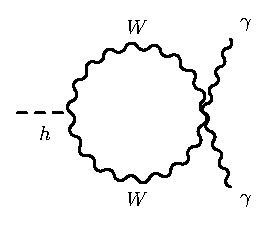
\includegraphics[scale=0.25]{hgg}
\end{minipage}
\end{frame}

\begin{frame}
 \frametitle{ttH @ LHC 8 TeV}
\begin{center}
\includegraphics[scale=0.25]{sigma}
\end{center}
\end{frame}


\begin{frame}
 \frametitle{ttH}
\begin{itemize}
 \item \textbf{ttH is difficult}: cross section $\approx$ 1/100 of $gg\rightarrow H$ (gluon-gluon fusion)
\end{itemize}
\begin{minipage}{.45\columnwidth}
 \includegraphics[scale=0.26]{Higgsxs}
\end{minipage}
\begin{minipage}{.45\columnwidth}
 \includegraphics[scale=0.26]{br}
\end{minipage}
\begin{itemize}
\item The final state is very complex, considered the presence of a
high number of jets
\item The experimental challenge here is to fully exploit the whole detector
and advanced techniques like b-tagging in order to obtain a relevant statistical significance.
\end{itemize}
\end{frame}
\begin{frame}
\frametitle{Sensitivity to new top-partners}
\begin{itemize}
\item Within several theories beyond the SM there are candidates for new heavy colored states: extra ``up-type`` quarks with
\textbf{vector-like couplings}\footnote{arXiv 1204.0455v1 \itshape{Higgs boson production via vector-like top-partner decays}:
Azatov et al }
\item Vector-like means that both chiralities have the same transformation
properties under SU(2) X U(1)
\pause
\item $T\rightarrow th, tZ, Wb$
 \item If top partners exist the ttH cross section can be increased even by a factor 10,
depending on the heavy top mass
\item Given that, with the current amount of data, we will be able
to exclude or confirm the existence of these particles up to ∼400 GeV of mass.
\end{itemize}

\end{frame}







% qui cominciano le slides di back-up
%\appendix
%\newcounter{finalframe}
%\setcounter{finalframe}{\value{framenumber}}
%\begin{frame}
% \frametitle{Back-up}
%\end{frame}

%\setcounter{framenumber}{\value{finalframe}}
\end{document}